% Created 2022-07-22 Fri 17:10
% Intended LaTeX compiler: pdflatex
\documentclass[11pt]{article}
\usepackage[utf8]{inputenc}
\usepackage[T1]{fontenc}
\usepackage{graphicx}
\usepackage{longtable}
\usepackage{wrapfig}
\usepackage{rotating}
\usepackage[normalem]{ulem}
\usepackage{amsmath}
\usepackage{amssymb}
\usepackage{capt-of}
\usepackage{hyperref}
\author{Eshan Ramesh}
\date{July 18th 2022}
\title{A deep dive into the OFDM implementation in GNURadio}
\hypersetup{
 pdfauthor={Eshan Ramesh},
 pdftitle={A deep dive into the OFDM implementation in GNURadio},
 pdfkeywords={},
 pdfsubject={},
 pdfcreator={Emacs 29.0.50 (Org mode 9.5.4)}, 
 pdflang={English}}
\begin{document}

\maketitle
\tableofcontents


\section{Introduction}
\label{sec:org9bfc007}
GNURadio (GR) provides the \texttt{OFDM Transmitter} and \texttt{OFDM Receiver}
blocks to do orthogonal frequency division multiplexing. These blocks
are hierarchical, meaning that they're really composed of other (C++)
blocks internally. Indeed, both of these blocks are written in python
and simply describe connections between blocks. Because of this, there's a
great deal of implementation detail in the source code of these blocks
that is poorly documented in a simple and clear manner. This article
is an in-depth explanation of the OFDM implementation.

I'll shortly be working on updating the GR wiki and block
documentation with these notes, but for now they'll stay here. What I
won't be covering in depth is the mathematical basis for much of OFDM,
instead I write about these ideas mostly on my personal \href{https://notes.esrh.me/}{wiki}, although
the standard texts in telecom certainly do a better job. I'll try to
include a bare minimum here, and link to my wiki articles or other key
sources when possible. \href{https://notes.esrh.me/orthogonal\_frequency\_division\_multiplexing.html}{Start here}.

\subsection{High level introduction to the OFDM idea}
\label{sec:org5ceec2c}
Orthogonal frequency division multiplexing is a multi-carrier scheme
that's fairly widely used today, especially in WiFi and LTE.

This multi-carrier property just means that instead of transmitting a
signal at one frequency (on one "carrier wave"), we transmit on many
sub-carriers spaced apart by a little bit of bandwidth.

The core of the idea that makes OFDM special is the technique by which
it makes these subcarriers independent (or, orthogonal), which boils
down to computing the IFFT of the signal at the reciever and adding a
cyclic prefix in between each set (determined by the size of the FFT)
of data pieces. I go into much more detail about why this leads to
interesting properties in \href{https://notes.esrh.me/orthogonal\_frequency\_division\_multiplexing.html}{another article} I wrote about
\section{Transmission}
\label{sec:orgea75003}
The following is a mostly faithful reconstruction of the transmission
scheme given in \texttt{gr-digital-python/digital/ofdm\_txrx.py}.
\begin{center}
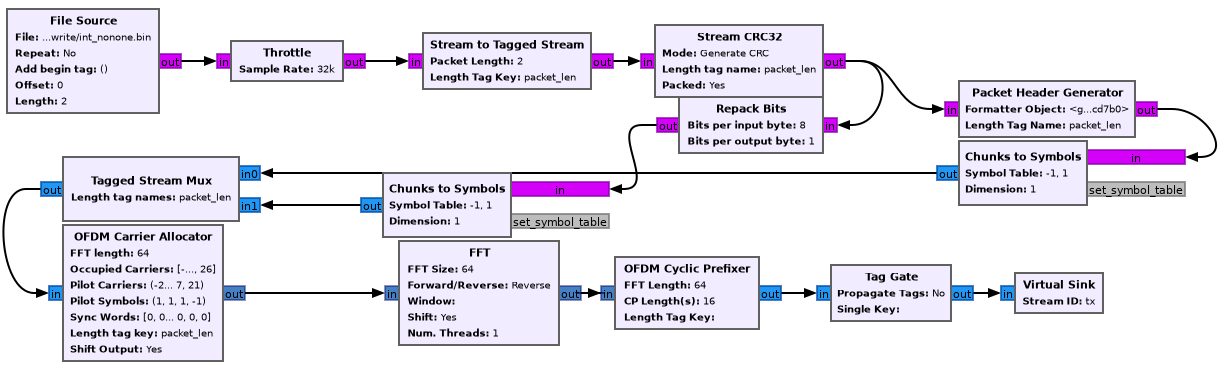
\includegraphics[width=\textwidth]{./images/ofdm_tx.png}
\end{center}

For the sake of the narrative, we'll take it step by step and
introduce the parameters to each block as we get there.

\subsection{File source}
\label{sec:orgc15f198}
For the purposes of this whole example that we'll follow through the
chain, let's assume we want to transmit some number of bits, say 16 of
them (we'll see why this number is convenient shortly).

For simplicity, let's say all these bytes are just 1 bits, so
You might generate a file to be used with this block with a bash call
to like \texttt{printf '\textbackslash{}xFF\textbackslash{}xFF' > test}, but pick your poison.

Set the length to 2, since we want 2 bytes.
\subsection{Stream to tagged stream}
\label{sec:org8f46e6f}
Classic streams in GR are just streams of bytes with no information or
grouping. We however, would like to group the bytes together in a
flexible way (meaning that we should be able to increase the size of a
group).

The technique for doing this is attaching a "tag" every \(n\)
samples,. This tag says nothing but the length of the group following
it. Really the reason this is necessary is so that C++ programs can
allocate memory for a buffer large enough to do processing on that
group, before recieving the data. See the \href{https://wiki.gnuradio.org/index.php/Stream\_Tags}{GRwiki article} on tagged
streams. Stream tags are quite flexible, and we'll see them again for
other uses. Fundamentally, tags are just a pair of key and value,
where both are polymorphic-types (\href{https://wiki.gnuradio.org/index.php?title=Polymorphic\_Types\_(PMTs)}{PMT's}).

For our example, since we want to transmit 2 bytes, we'll set the
length to 2.

\subsection{Stream CRC32}
\label{sec:orgc33ea1f}
This block simply adds the CRC32 error-detection code to the end of
the data. The reasons why CRC32 tends to be pretty good for OFDM
bursts, and the implementation of the algorithm are explained pretty
well by \href{https://en.wikipedia.org/wiki/Cyclic\_redundancy\_check}{this wikipedia article}.

The CRC32, as the name suggests, adds 32 bits (\(\frac{32}{8} = 4\)
bytes) to our data, bringing the length up to 6 bytes.

\subsection{Header generator}
\label{sec:org3a6bdf6}
The data coming out of the tagged stream block splits here. We'll talk
about the header generation first.

Let's take some time to talk poorly-named jargon for a second:

\begin{description}
\item[{OFDM frame/burst}] a set of some number (as many as necessary) of
OFDM symbols and other stuff
\item[{OFDM symbol}] a set of \(n\) (determined by the size of the FFT)
complex symbols
\item[{complex symbol}] an atomic piece of encoded data. for more
information about why you can hold signals as complex numbers, see
\href{https://notes.esrh.me/quadrature\_signal.html}{my article} on quadrature signals.
\end{description}

The "other stuff" included in an OFDM frame are 3 extra OFDM symbols,
the header OFDM symbol, and two "sync words" that are known by the
reciever as part of some standard. We'll see the generation of the
sync words and their usage for time and frequency synchronization
later on in the reception section.

The header OFDM symbol (before modulation) contains three pieces of data:
\begin{enumerate}
\item 12 bits for the length of the packet (here, 6 (including the 4 extra from the CRC))
\item 12 bits for the header number, which is incremented after every packet (modulo xFFFF)
\item 8 bits of CRC computed from a combination of the above numbers.
\end{enumerate}

We must encode these bits one way or another, but the number of bytes
(and thus complex symbols) used to encode these bits depends on the
\href{https://notes.esrh.me/linear\_modulation.html}{modulation} scheme used, and in particular, the number of bits we can
encode in a specific complex symbol.

Classically, in the standard, we encode everything in the header with
BPSK, binary phase shift keying, which essentially encodes one bit in
the phase of one complex symbol, and gives all-real complex symbols.

With BPSK, each byte will only have its LSB representing actual
data. With QPSK, which can encode 2 bits per complex symbol, the
lowest 2 bits in the byte represent data, and so on. The reason we
have to do this is because next, we will be mapping bytes to complex
symbols, but it wouldn't do to pack a byte full of data when we can
only encode 1 of the 8 bits into a symbol to transmit.

In sum, at worst (BPSK), we have 32 bytes (although, each byte only
has one bit of data) of header data, but we will send this as one OFDM
symbol on it's own. In IEEE jargon this is either called the header or
the SIGNAL symbol, and in practice also includes information like data
rate (can't just waste 20 bits, can we?).

A particularly sharp reader might notice that we encode the packet
length as 6, even though the real packet length will be 6 * 8 = 48
complex symbols. This is fine, because the factor of 8 is compensated
on the receiver side in the OFDM serializer block, which we'll cover
shortly.

\subsection{Repack bits}
\label{sec:org47525ff}

Typically the CRC32 block is routed through a "Repack bits" block
before being converted to symbols.

The incoming data is usually a byte array that is packed full of data,
but we want each byte to represent just as many bits as we can encode
into a single complex symbol.

If we're using BPSK, then each byte should only have one bit of
data. The repack bits block takes a \(k\) and \(l\), and converts bytes
containing \(k\) bits of data into bytes containing \(l\) bits of
data. Thus for BPSK, we'd use \(k = 8, l = 1\), and for QPSK we might
use \(k = 8, l = 2\).

At \((8, 1)\), a byte array containing \texttt{[FF]} is transformed into \texttt{[1 1
1 1 1 1 1 1]} Similarly, A byte containing \texttt{[0F]} becomes \texttt{[0 0 0 0 1
1 1 1]}, where each of these 0s and 1s aren't bits, but \textbf{bytes with
the top 7 bits off}.

\subsection{Chunks to Symbols}
\label{sec:orga01474b}
Here we convert each byte into a complex symbol. This is done via a
symbol table, or a \emph{constellation}. I briefly discuss the ideas behind
constellation encoding \href{https://notes.esrh.me/phase\_shift\_keying.html}{here}, but the high level idea is to map each
bit, or sequence of bits, to a "location" on the complex plane, or a
pair of real and complex co-ordinates, so they can be transmitted as a
quadrature signal. This is possible since \(\sin\) and \(\cos\) form
orthogonal bases for the signal space.

Constellations are typically quite specific. Points on the
constellation should be as far apart as possible, in order to minimize
the ambiguity when decoding any particular recieved complex
symbol. However, the distance of a constellation point from the origin
affects the energy (magnitude of the resulting symbol) required to
transmit, and so this must be considered as well.

Here we use binary-phase-shift-keying for the payload's encoding,
although the IEEE standard suggests QPSK for a higher data
transmission rate. In BPSK, resulting complex symbols are real, and
the real part is 1 if the bit is 1, and -1 if the bit is 0.

In gnuradio, the BPSK constellation points are obtained as:

\begin{verbatim}
from gnuradio import digital
header_mod = digital.constellation_bpsk()
points = header_mod.points()
\end{verbatim}
\subsection{Tagged stream mux}
\label{sec:orgf7745ff}
This block combines two streams in order. The output is the first
stream followed by the second stream.

\subsection{OFDM carrier allocator}
\label{sec:org1ec00f0}
Now, we have a long stream of complex symbols, (80, to be exact), and
we must transform them into vectors of what to load into each
frequency. Assuming that we are using 64 subcarriers (IEEE standard),
we expect to produce a vector of \(n\) samples, which are each arrays of
64 complex numbers, where \(n\) is the number of OFDM symbols we're
sending in the frame.

Here, we have one OFDM symbol for the header, one symbol for sync word
1, and another symbol for sync word 2, and one symbol for data and the
CRC32 code. The structure of each sync word is given below.

In OFDM, although we get 64 subcarriers to transmit on, payload OFDM
symbols only get 48.

The \href{https://notes.esrh.me/ieee802\_11.html}{IEEE 802.11a} standard suggests transmitting on subcarriers from
-26 to +26, for a total of 52 subcarriers. That's what we'll use for
now in our example. This subcarrier indexing is relative to some
central carrier frequency at index 0. The frequency spacing between
subcarriers will be determined by the size of the FFT.

The bottom 6 and top 5 subcarriers are meant to be left empty
according to the IEEE standard. This is generally to prevent excessive
out-of-band emission. It's also convenient when applying a low-pass
filter to the signal.

Additionally, the zero-subcarrier is left null. This is again a
measure for hardware devices that have interference at the carrier
frequency, specifically \href{https://en.wikipedia.org/wiki/Direct-conversion\_receiver}{synchrodynes} which have an oscillator tuned to
the carrier frequency.

Finally, the pilot subcarriers, (-21, -7, 7, 21) contain
receiver-known data as well. These sequences are used for a wide
variety of purposes, and it's protocol dependent. Here, the pilot
sequence is (1, 1, 1, -1), one symbol per pilot tone.

It's important to note that the preamble (combination of the sync
words) don't follow these rules. The sync words transmit
non-pilot sequences on the pilot subcarriers.

The reason why we chose to transmit 2 bytes is now clear. After CRC,
we have 6 bytes, and \(6 * 8 = 48\) bits, if you use BPSK to encode one
bit to one complex symbol, this is exactly as many as we can fit into
one OFDM symbol. Using QPSK as the IEEE standard suggests would let
you fit twice as much data.

The operation of the OFDM carrier allocator block is now fairly simple
to explain.

\begin{enumerate}
\item Copy each sync word into the output buffer (each are 64 complex
symbols) straight
\item For each of the header and data symbols (remember, we muxed them)
\begin{enumerate}
\item Copy a symbol to each of the occupied carriers
\item Fill in the pilot carriers with the pilot sequence
\end{enumerate}
\item Return the size of the vector to ensure it's formatted correctly
\end{enumerate}

Because we have 2 sync words, 1 header, and 1 data symbol, we'll have
4 OFDM symbols in a single vector sample [see below for a
clarification on this] now.

\subsubsection{Sync words in OFDM synchronization}
\label{sec:org20a85f2}
The idea of "sync words" are fundamental to wireless
communication. The receiver is only able to equalize for environmental
and interference conditions (the "channel"), when there is some data
transmitted that is known to both the transmitter and receiver.

Sync words may also be used for detecting when the packet starts at
all, as well as compensating for a constant (across subcarriers)
frequency offset, the \emph{carrier frequency offset}.

Typically, these sync words have some clever properties that make
doing these easier. I'll outline the generation of each of these sync
words briefly.

\begin{enumerate}
\item Sync word 1
\label{sec:orgd89c667}
Sync word 1 is generally used for timing estimation (i.e when does our
data start), which is sent first since you can only pick up data
following it.

In 1997, Schmidl \& Cox proposed using a sync word that had identical
first and second halves. What is actually in these halves isn't so
relevant, but they should have constant transmit energy.

From a property of the discrete fourier transform, the classical way
to produce a time-domain signal that is duplicated around its center
is to take the DFT of a signal that has real-only data on even
frequencies (assuming a symmetric fft frequency ordering scheme
starting from \(-k\) and ending at \(k-1\) inclusive). To be more
specific, this holds when the signal has hermitian symmetry and the
right parity. In the interest of space, I'm not including the proof
here, but it can be found in 8.6.4 (p. 653) of \emph{Discrete-Time Signal
Processing} by Oppenheim \& Schafer.

We can produce this sync word with:
\begin{verbatim}
list(map(lambda x: np.sqrt(2) * np.random.choice([-1, 1])
         if (x in oc[0]+[-21, -7, 7, 21] and x % 2 == 0)
         else 0,
         range(-32, 32)))
\end{verbatim}
where \texttt{oc[0]} is a list of occupied carriers.

\item Sync word 2
\label{sec:org2b1fd95}
Sync word 2 is used for channel estimation and coarse frequency
offset. Computed via

\begin{verbatim}
list(map(lambda x: np.random.choice([-1, 1])
         if x in oc[0]+[-21, -7, 7, 21]
         else 0,
         range(-32, 32)))
\end{verbatim}

Note that the second sync word indeed has higher magnitudes, and thus
transmit energy, but it will prove to be useful during reception.
\end{enumerate}

\subsubsection{Streams vs vectors}
\label{sec:orgf664a89}
In GR, streams and vectors are the two main types of data passing
techniques. Streams pass each sample individually, whereas vectors
contain some number of samples in a vector.

In this way, blocks that operate on vectors (notably, the FFT block),
should be thought of as doing a parallel computation.
\subsection{FFT}
\label{sec:orgf7f0344}
This block simply applies the inverse \href{https://notes.esrh.me/fourier\_transform.html}{discrete fourier transform} in
parallel (operates on a vector) to each of the 64-length OFDM symbols.

The output will therefore also be 64-length time-domain OFDM symbols,
although the meaning of the word is now slightly different. The
inverse fourier transform is used here, expecting that the resulting
time domain signal will be cyclically prefixed.
\subsection{OFDM cyclic prefixer}
\label{sec:org3873523}
This block applied a cyclic prefix to each item in the vector input. A
cyclic prefix is simply prefixing a block by some number of
time-domain symbols from the end of a 64-length block.

The cyclic prefix is the core of the OFDM idea, and has deep
implications for equalization at the receiver. I'd recommend my
article on OFDM, or the paper "Wireless multicarrier communications"
by Wang \& Giannakis (2000).

The high level idea, skipping a fair bit of linear algebra, is that
adding the cyclic prefix turns the linear convolution of the data with
the channel (since the output of a linearly time invariant channel is
determined via linear convolution) into a circular convolution. As it
would turn out, the matrix that does circular convolution turns out to
be diagonalizable in the Fourier basis, which implies a removal of
inter-symbol interference by pre and post multiplying by the inverse
DFT and DFT matrices, as well as cheap equalization techniques.

As for the implementation of the cyclic prefixer block, I'll only
explain it in a bit of a limited scope. The block has two operating
modes, one meant to be used before the carrier allocator in the stream
domain "packet mode", and the other meant to be used after the FFT, in
so called "freewheeling mode." I'll only cover the second, which is
enabled by not specifying a length tag.

Additionally, the block supports the application of the raised
cosine pulse shaping filter parametrized by a rolloff length, but this
is typically unnecessary and is indeed set to a default of 0.
\textbf{*}
\subsection{Output}
\label{sec:org4f7013e}
Quick picture of what you might expect to see at the transmission end
of the OFDM chain.

\begin{center}
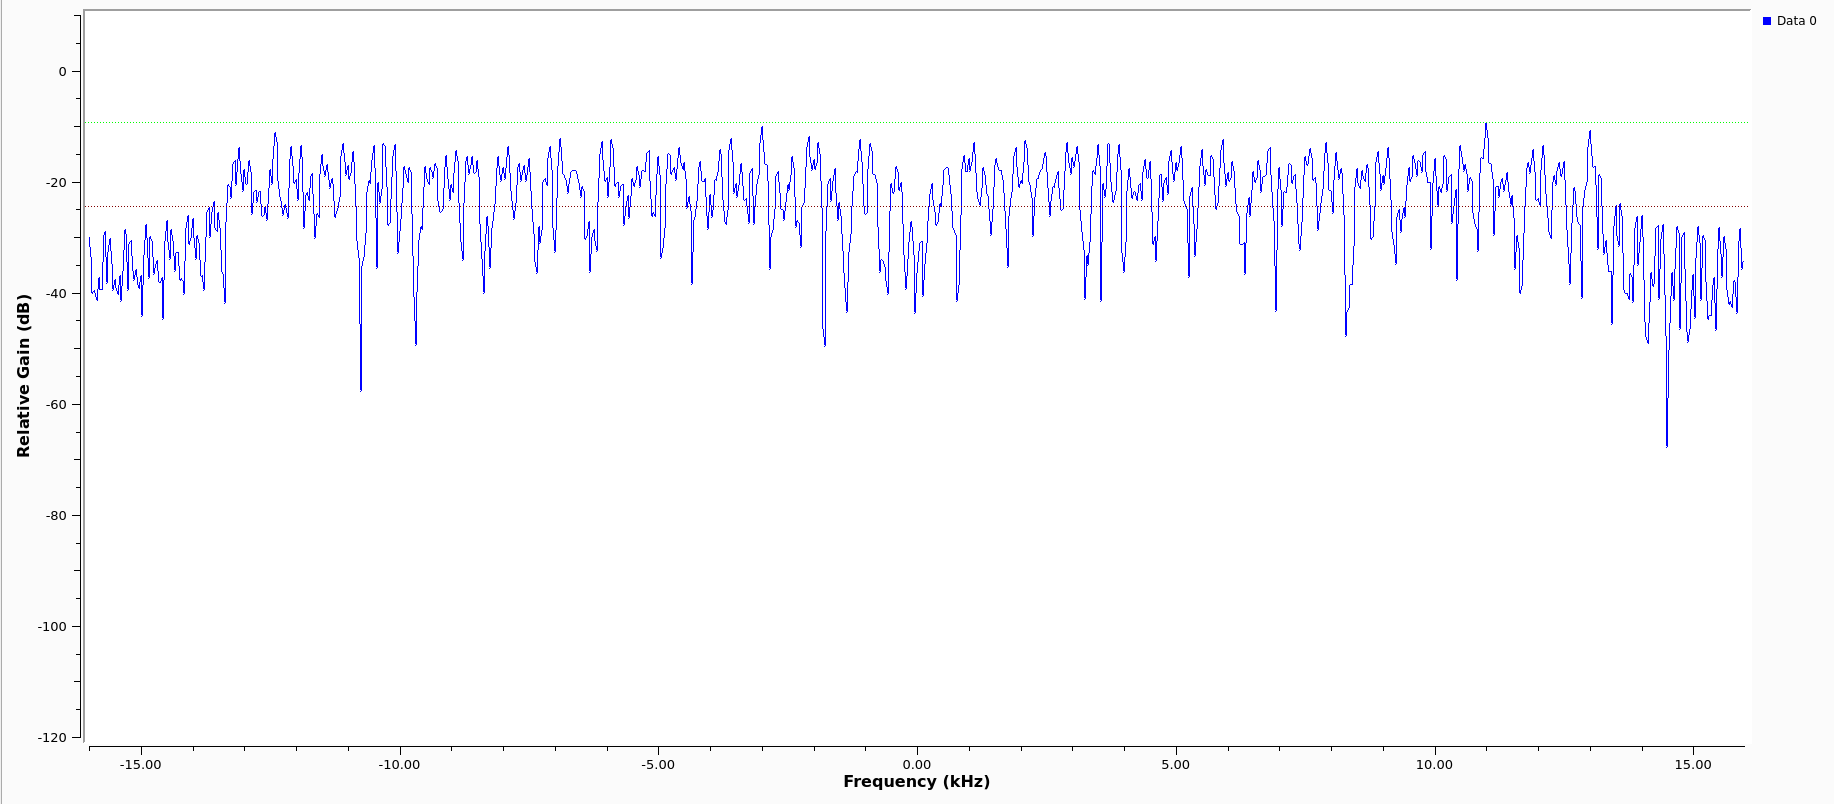
\includegraphics[width=\textwidth]{./images/frequency.png}
\end{center}

We can clearly see the side lobes due to null subcarriers.
\section{Reception}
\label{sec:org02e0524}
Here's an expansion of the reciever block, which is significantly more
complicated than the transmitter.

\begin{center}
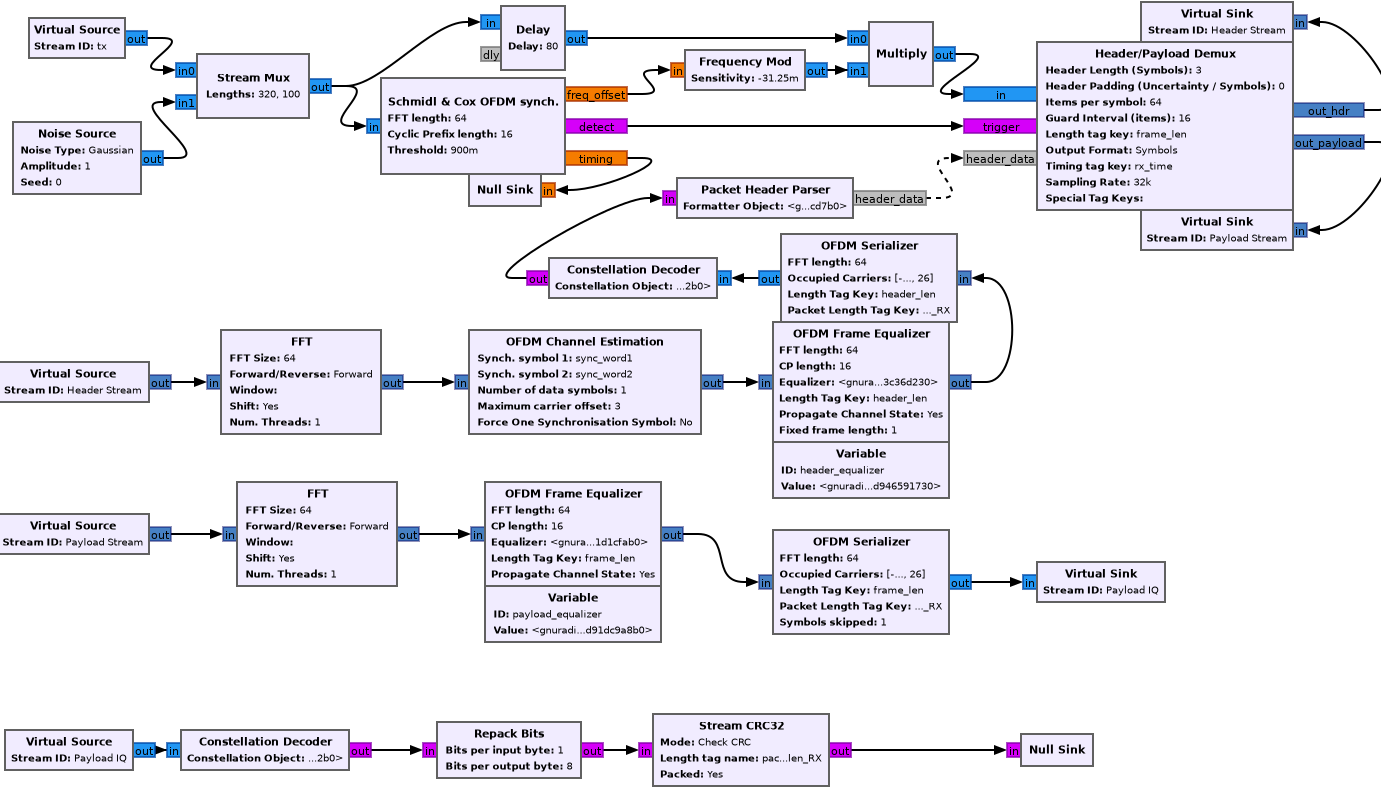
\includegraphics[width=\textwidth]{./images/ofdm_rx.png}
\end{center}
\subsection{Schmidl \& Cox}
\label{sec:orgf812dcc}
The first step in decoding an OFDM burst is to figure out when it
starts. This block uses the strategy given by Schmidl \& Cox in their
1997 paper "Robust Frequency and Timing Synchronization for OFDM."
There are two things that the algorithm achieves. The first is
determining when the frame starts of course, but the second is coming
up with a fine frequency offset measure that in effect cancels out the
short-term carrier frequency offset, in which the carrier frequency is
slightly off due to a slight, constant time offset in the oscillator.

\subsubsection{Timing sync}
\label{sec:org76ea7a8}
The timing synchronization portion relies on the property of the first
sync word to be symmetric, as in its first half should be exactly
equal to its second half.

We also know how long the whole symbol is, 64 complex
samples. Therefore, we can figure out when we're looking at the sync
word by \href{https://notes.esrh.me/autocorrelation.html}{autocorrelating} the incoming signal with a signal that's
delayed backwards in time by 32 samples. Recall that autocorrelation
is really just multiplying with the conjugate, so clearly we'll get
the highest value when the two signals "match up".

The schmidl and cox block is a hierarchical block itself which does
this.
\begin{enumerate}
\item Delay the signal by 32 samples, take its complex conjugate
\item Multiply with the non-delayed signal
\item Low-pass-filter to smoothen the data
\item Compute the magnitude squared of each complex symbol
\item Divide by the square of the magnitude squared of the non-delayed
signal, also low-pass-filtered. This normalizes the correlation
metric since you're dividing out one part of the original multiplication.
\item Find the plateau of the result of 5.
\end{enumerate}

\begin{center}
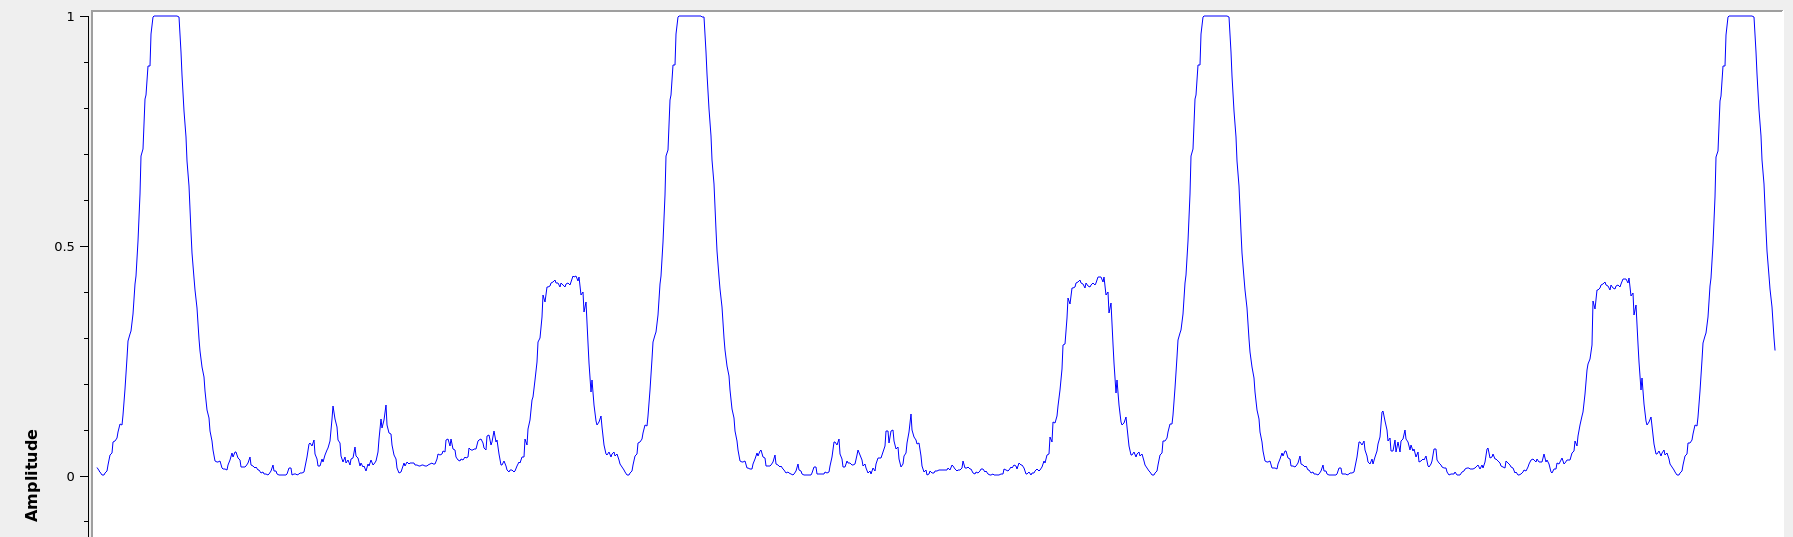
\includegraphics[width=\textwidth]{./images/sc.png}
\end{center}

You can observe a graph showing autocorrelation peaks like the above
by defining the flag SYNC\textsubscript{ADD}\textsubscript{DEBUG}\textsubscript{OUTPUT} in the source file
\texttt{ofdm\_sync\_sc\_cfb\_impl.cc}, editing the corresponding block \texttt{.yml}
file, and recompiling gnuradio. This is handy for fine tuning the
necessary threshold for plateau detection. The graph above is recorded
during a transmission with USRP 2901 SDRs. I believe the smaller peaks
are due to the fact that our payload OFDM symbol is all ones, and is
therefore also close to having identical first and second halves,
except for the pilot symbols.

\begin{enumerate}
\item Plateau Detection
\label{sec:org3514fb5}
Step 6 has some nuance. You will see that the S\&C block outputs a
\emph{byte} on the "trigger" port which is wired to the plateau
detector.

The plateau detector accepts a series of floats, the output will be a
byte array filled with as many zeros as samples are given, and a 1 at
the index at which the plateau was detected.

Plateau detection works by looking for data above a certain
threshold. This threshold must be heuristically determined (i.e trial
and error) based on channel conditions. Once a data point above the
threshold is found, we continue iterating until we find the first data
point below the threshold. If the difference between the indices of
these two points is bigger than one (there wasn't just an outlier),
then we set the index corresponding to the midpoint between the two
points to 1 in the output byte buffer.

I'm not entirely certain why the center of the plateau is chosen
instead of the flank start.
\end{enumerate}
\subsubsection{Fine frequency offset}
\label{sec:org0cc8a98}
The key observation is that the frequency offset we're trying to
eliminate, the carrier frequency offset, will result in accumulated
phase shifts over time. Since the first sync word is identical in the
first and second half, all we need to do is compare the recorded
phases in the first half and the second half.

This is done in much the same way as the timing sync computation.
\begin{enumerate}
\item Compute the correlation between the signal and the signal delayed
by half the length of the OFDM symbol (32 samples)
\item Low-pass filter the result of the correlation, and compute the arg
(a.k.a arctan, angle or phase)
\item Output the latest arg result from 2 when a peak is detected by the
plateau detector in the timing sync path.
\end{enumerate}

It is critical to note that the output of this block isn't actually
"frequency offset" as the name suggests, but phase offset instead,
\(\hat{\phi}\) in the paper if you're familiar with it.

\begin{enumerate}
\item Applying the frequency offset
\label{sec:org5a21490}
Actually modifying the signal using the frequency offset metric
computed earlier is not immediately straightforward.

The first issue is that because the plateau detection is done using a
signal delayed by N/2 samples, by the time we've detected the frame,
we must have finished looking at the (undelayed) second half, and
compared it to the (delayed) first half. So, when we actually want to
use the frame, we have to backtrack, by using a signal delayed by the
length of the whole sync word. Recall that the sync word is 64
samples, but there are 16 extra samples from the cyclic
prefix. Therefore, we have to use the signal shifted by 80 samples.

The second issue is that the normalized frequency offset has to be
applied to the signal. In the paper, the authors write (p. 8) that the
frequency must be offset by \(\frac{\hat{\phi}}{\pi T}\) by multiplying the
signal with the complex waveform \(e^{-j2t\hat{\phi}\frac{1}{T}}\) where
\(\phi = \Delta f \pi T\) (eq. 39). Substituting, we get \(e^{-j2\pi t
\Delta f}\)

Things can get a bit tricky here. In the paper, \(T\) refers to the
length of the OFDM symbol in \emph{complex symbols}! The index \(t\) doesn't
refer to a time index in say, seconds, but rather indexes the complex
symbols, and goes from \(0 \dots T\) which is in fact equal to the size
of the FFT. Similarly, \(\Delta f\) does not refer to actual bandwidth
in Hz, but is instead normalized to the spacing of the carriers
themselves.

The frequency mod block computes the waveform \(e^{jk\phi}\), where \(k\)
is the sensitivity parameter. Really, this block performs general frequency
modulation of a signal that varies, but in for this case this
simplification works fine. Solving for \(k\), we see that it must be
\(\frac{-2}{T}\) in order to match the required waveform.

In summary, all we really need to do is take the phase offset
estimate, produce a waveform that will correct the signal via
frequency modulation, and the multiply that waveform with a
sufficiently delayed version of the signal.

We have to be a little careful here as well. Delaying a signal by 80
samples has the effect of prepending 80 zeros to the front of the
data. With 4 total OFDM symbols, that's 320 + 80 = 400 items. The
Schmidl \& Cox block however, receives a signal of length 320, and so
the frequency mod sinusoid is also of length 320. Multiplying the two
in GR, the longer signal will get truncated from the front, which
means that you will lose a data payload symbol, \emph{not good!}

This isn't a real problem if you repeat your frames over and over
again, or if you use a real SDR that is always collecting samples, but
can be hard to debug in a pure, oneshot simulation. The solution is
the mux the input tx stream with an extra 80 items of noise or
constant at the end of the signal data.
\end{enumerate}
\subsection{Header/Payload Demux}
\label{sec:orgbbb143d}
The HPD block is a very complex mechanism for parsing burst
transmissions like OFDM. The block acts like a state machine, with the
default state being waiting for the data on the trigger port. An
important distinction when discussing the parameters of this block is
items vs symbols. Items refers to the actual complex samples coming
from the radio. Symbols on the other hand, refers to OFDM symbols
here. Therefore, our items\textsubscript{per}\textsubscript{symbol} should be fft\textsubscript{len}, 64. Ensure
that the block is set to output symbols, because this is what every
OFDM block expects downstream.

\subsubsection{Trigger state}
\label{sec:org215c938}
In the default state, we search the byte array sent to the trigger
port, and find the index (i.e offset) until the first set byte. From
here, switch to the header state.

\subsubsection{Header state}
\label{sec:org8e9503a}
Header state copies a certain parametrized number of full symbols (64
items) into the header port, and switches to the msg wait port.

Here, we wait for a message to be sent to the message in port. This
state does nothing, and will not be exited until
parse\textsubscript{header}\textsubscript{data}\textsubscript{msg}() is called to set the state to either
HEADER\textsubscript{RX}\textsubscript{FAIL} or HEADER\textsubscript{RX}\textsubscript{SUCCESS}.

This method waits for a PMT (polymorphic type) dictionary, where the
key is an interned string corresponding to the length\textsubscript{tag}\textsubscript{key} and the
value is a long representing how many OFDM symbols are in the current
frame (which recall, is encoded in the header symbol). Alternatively,
you may also just send a single PMT long, in which case this is
interpreted as the length of the payload. A PMT that is parsed in
either way sends us to the success state.

A PMT that is instead PMT\textsubscript{F} (the token failure placeholder) sends us
to the failure state. Two extra cases can send us to the failure
state, one in which the payload length is negative, and one in which
the payload length is greater than the half the output buffer. By
default, this means that you are capped at 64 payload symbols per
frame, if your items are indeed complex.

For our purposes in this example, it is entirely possible to write a
block to, on receiving any data, sends a message with value 1, since
we know how many OFDM symbols are in the payload, but in practice the
number of payload symbol varies depending on how much data we need to
transmit.
\subsubsection{Header RX Success}
\label{sec:orge1da158}
Transitional state that consumes the header items and any
padding. This is to make the in buffer aligned perfectly with the
payload on the next work iteration.
\subsubsection{Payload}
\label{sec:org7689969}
Simply copy the number of items determined in the header state to the
payload output port. If the output symbols option is toggled, then the
output will be symbols, therefore the payload will be a vector of
length payload\textsubscript{length} (here 1), and each element is another array of
64 complex numbers).

It's super important to realize, especially in simulation, that the
payload state will only trigger when there actually enough samples as
we're expecting (given the frame length from the message).
\subsection{Header chain: FFT}
\label{sec:org7a10169}
We'll now discuss the "header chain", or the path from the header out port
of the HPD, to the message in port of the same demux block.

Currently, our 64-length vector of symbols (currently 3 in the
example, 2 syncs and 1 header) is still in the time domain. However,
they were encoded in the frequency domain, so we convert from time to
frequency with a forward FFT block.
\subsection{Header chain: OFDM Channel estimation}
\label{sec:org26cdce0}
Here, we use the two sync words in order to compute the coarse carrier
offset and "channel taps" (the frequency response of the channel
across subcarriers). The channel taps specifically are critical to
know because that's how we equalize the signal to get our data out.

The channel taps are already corrected by the carrier offset.

The output vector will be missing both sync words, so only the header
is left. The channel estimation done results in a 64-length complex
vector, which is added to the vector as a tag, with key
\texttt{ofdm\_sync\_carr\_taps} and the carrier offset is added to the vector as
a tag with key \texttt{ofdm\_sync\_carr\_offset} and is a long.

\subsubsection{Carrier offset}
\label{sec:orgdab2149}
Carrier offset is computed in one of two ways, depending on how many
sync words are supplied.
\begin{enumerate}
\item 2 sync word case
\label{sec:orgb595dc8}
Computation follows the same procedure from the schmidl and cox block.
We iterate through some range of possible carrier offsets, compute the
\(B_g\) metric (eq 41), and find the \(g\) that maximizes it iteratively.
\item 1 sync word case
\label{sec:orgdb7ae4e}
In this case, the block will fill a new, artificial kind of sync word
by computing the differences between every item and the item two
samples ahead of it. Of course, this means there are two fewer (62)
items in the new word, so there are 2 zeros left behind at the end.

Next, we do a very similar correlation procedure between the original
word and the artificial one. First iterate through \(g\) for possible
carrier offsets, and find the \(g\) that gives the maximum sum of products
between the \(j\)th item of the known sync word and the \(j + g\)th item
of the artificial one.
\end{enumerate}
\subsubsection{Channel taps}
\label{sec:org86bec03}
To compute channel taps, we'll use the second sync word if it exists,
otherwise just use the first one.

GR does channel estimation using a very simple technique, in which
every item received in the sync word is just divided by the known item
at that index.

We must offset the taps using the carrier offset computed
earlier. This is simply done by only computing the channel taps
starting at the offset frequency if positive, or ending \(g\) items
short of the end of symbols if negative. While doing the division, we
compare every \(i\)th received element with the \(i - g\)th element, where
\(g\) is the offset in carriers.

In the one-sync word case, where we're forced to use sync word 1, we
have to deal with the fact that there is only data on the even
frequencies. Because everything else is 0s, the channel taps
(received/reference) will also be 0s on the odd frequencies. To
interpolate, GR uses the naive strategy of setting every odd frequency
to the even frequency immediately behind it.

In the source file for ofdm\textsubscript{chanest}\textsubscript{vcvc}, there's a TODO left for
implementing red noise thresholding.
\subsection{Header chain: Frame equalizer}
\label{sec:org8eb8388}
This block equalizes an OFDM frame (a sequence of OFDM symbols) using
the tags produced by the chanest block earlier. To be a bit more
accurate, the block itself doesn't do the equalization, but uses an
equalizer object that the user passes in.

One extra tag is added to the vector output, containing the number of
symbols in the frame.

Before using the equalizer object, a few things are done:
\subsubsection{Offset correction}
\label{sec:org4c6ec8c}
\begin{itemize}
\item If the offset \(g\) is negative, then set \(g\) zeros in the beginning
of the output, and copy the whole header shifted forward by \(g\)
items.
\item If the offset is positive, we need to shift back. Set the last \(g\)
items to be zeros, and then copy the header starting at the offset
straight into the output buffer, dropping \(g\) items at the end to
avoid writing into the zeros.
\end{itemize}
\subsubsection{Phase correction due to offset}
\label{sec:orgb431808}
The carrier offset (an offset in frequency) will also result in a
phase offset. This is also corrected. For each OFDM symbol, every item
is multiplied by a factor of \(\exp{j-2\pi g (i + 1) \frac{N_{gi}}/{N}}\)
where \(g\) is the offset, \(N_{gi}\) is the length of the guard interval,
\(N\) is the fft size, and \(i\) is the index of the current OFDM symbol.

Looking at this phase correction, the point to notice is the the phase
correction for each OFDM symbol changes over time, and indeed
accumulates until it wraps around \(2\pi\). Second, the speed at which
the phase correction changes depends on the size of the carrier
offset. If the carrier offset in 1, then the phase correction factor
wraps around every 4 symbols, but if 2, then it wraps around every
other symbol.

\subsubsection{Equalization}
\label{sec:orgf89caec}
There are two variants of equalizers implemented in GR at the time of
writing, static and simpledfe. We'll discuss simpledfe (simple
Decision Feedback Equalizer) here.

There are essentially two parts to how the equalizer works. The first
is the pilot-based channel modification, and the second is the
constellation mapping.

For each symbol \(i\) and for each subcarrier \(k\) in each symbol, if it is a
pilot carrier then we update the channel state for \(k\) to be

\begin{equation}
\alpha * H[k] + (1-\alpha) * \frac{s_{i, k}}{p_j}
\end{equation}

Where \(H\) is the frequency response of the channel, \(\alpha = 0.1\) is
a constant, \(p_j\) is the pilot symbol corresponding to the \(k\)th
index, and \(s_{i,k}\) is the received symbol.

Note that this modified channel is written back to the same tag that
the channel taps were found on.

If the subcarrier is not a pilot subcarrier, then we update the
channel in a similar way.

First, let the equalized symbol just be \(\frac{s_{i, k}}{H_k}\). Next,
we use the constellation mapper to essentially "snap" the complex item
to a complex item that we know, in this case either -1 or +1.

Now that we know what this symbol really was (the decision), we can
use this feedback to update our channel slightly, via the same
equation above, just using the snapped complex number instead of the
pilot symbol.

If soft output is enabled (not by default), then the non-snapped
output is outputted, otherwise the snapped, perfectly constellation
aligned output is used.

Before propagation, the new output is also corrected for phase shift.
\subsection{Header chain: OFDM Serializer}
\label{sec:orgd9b6bad}
This block undoes the carrier allocation, and pulls out the data from
each successive symbol's data subcarriers and strings them together
into a stream.

There are some easy footguns to make here related to tags, so again
I'll try to be very specific.

This block takes in two different length tags.
\begin{itemize}
\item "length tag key" is the tag that is \emph{used}. The previous block
writes a tag
\item "packet length tag key" (packet\textsubscript{len}\textsubscript{tag}\textsubscript{key}) and this refers to the
\emph{stream length} of the output stream. This block is a subclass of
the tagged stream block, which adds a tag to denote groups just like
it was done in the tx section. This tag only matters for the output!
\end{itemize}

The packet length tag key coming out is distinct from the packet
length tag key used in the transmitter. This is critical because the
same header\textsubscript{formatter} object is used in the transmitter and receiver
sections.

If the standard length tag key (i.e the frame length) is not provided,
then we simply recalculate the frame length.

The rest of the operation is straightforward. For every symbol in the
frame, pull out the complex items on each data subcarriers, making
sure to respect carrier offset.

Specifically, the \(i\)th output item corresponds to the \(s_{i, k +
g}\)th input item.
\subsection{Header chain: Constellation decoder}
\label{sec:org10241bb}
We now have complex packets, and must decode them back to bits (1-sig
bit bytes). This is done with the constellation decoder.

The simplest way to explain its operation is that we just calculate
the distance between the incoming complex item, and the constellation
points. We pick the closest one, and then output the byte
corresponding to that point. Notice though, that all the points will
already be perfectly snapped to one of the constellation points (so
the distance to the closest point will be zero) if we're using the
simple DFE described earlier.
\subsection{Header chain: Packet header parser}
\label{sec:org4dea553}
Does the opposite of the header generator.

The goal is to recover the length of the payload and the number of the
packet.

This is done by just picking out the data from the 32 bits, packet
length first, then header number, and finally the CRC. Then, we
compute the CRC and ensure that the data recovered is correct. If
its not correct, this results in an error.

If it is, then we put the payload length and the header number onto
the stream as tags, and then send a message containing every tag as a
PMT dictionary. These tags are not all necessary, but the payload
length one is essential for the HPD to continue operating.
\subsection{Payload chain}
\label{sec:org2a81b56}
The payload chain operates in pratically the exact same was the header
chain, so I won't duplicate that writing.

The only difference to speak of is that the channel estimation block
is not used. The reason is that the tag containing the channel's
frequency response is preserved through the header/paylod
demux. Therefore, we can just use the data on the tag.
\subsection{Repack bits}
\label{sec:org35200f7}
Every byte received only contains one bit of information, as a result
of our chosen modulation scheme. We should repack these bits into full
bytes.
\subsection{Stream CRC32}
\label{sec:org42748bf}
Every packet sent contained 4 bytes of CRC32. The CRC32 block checks
it to ensure that the packet was recovered correctly.

If it was, we're done!
\end{document}